\section{Espaço de recobrimento}
\label{espaco-de-recobrimento}

\begin{titlemize}{Lista de Dependências}
	\item \hyperref[homotopia]{Homotopia};\\ %homotopia
	\item \hyperref[grupo-fundamental]{Grupo fundamental};\\
    \item \hyperref[topologia-quociente]{Espaço quciente};
\end{titlemize}

Na topologia algébrica, espaços de recobrimento estão intimamente relacionados ao grupo fundamental: Todos os recobrimentos têm a propriedade de levantamento de curva e homotopia, portanto ao invés de acha uma homotopia em espaço original podemos verificar se existir uma homotopia num recobrimento que têm melhores propriedades topológicas. Por isso, os espaços de recobrimento são uma ferramenta importante no cálculo de grupos fundamentais.
\subsection{Espaço de recobrimento}
\label{espaco-de-recobrimento-def}
\begin{titlemize}{Lista de dependências}
	\item \hyperref[topologia-quociente]{Espaço quciente};\\ %'dependencia1' é o label onde o conceito Dependência 1 aparece (--à arrumar um padrão para referencias e labels--) 
% quantas dependências forem necessárias.
\end{titlemize}
\begin{defi}[Espaço de recobrimento]
Uma função contínua $p:E\rightarrow X$ é um \textbf{recobrimento} se para todo $x\in X,$ existe uma vizinhança aberta $U\subseteq X$ de $x$ e um conjunto de índices $\Lambda\ne \varnothing$ tal que 
$$p^{-1}(U)=\amalg_{\lambda\in \Lambda} V_\lambda,$$
onde $V_\lambda\subseteq E$ é um subconjunto aberto e $p|_{V_\lambda}:V_\lambda\rightarrow U$ é homeomorfismo.
\end{defi}

\begin{nota}
Introduzimos algumas terminologias: 
    \begin{itemize}
        \item $E$ é um espaço (total) de recobrimento.
        \item $U$ é um aberto uniformemente recoberto de $X.$
        \item $V_\lambda$ é uma placa de $U$ do recobrimento.
        \item A cardinalidade de $\Lambda$ é o número de folhas do recobrimento (veremos que $\# \Lambda$ não depende de $x$). 
    \end{itemize}
\end{nota}

\begin{ex}
A função $p:\mathbb{R}\rightarrow \mathbb{S}^1$ dada por $p(x)=e^{2\pi ix}$ é um recobrimento: dado $y_0=e^{2\pi i x_0}\in\mathbb{S}^1,$ e $U=\mathbb{S}^1\setminus \{-y_0\}$ nós temos 
$$p^{-1}(U)=\amalg_{k\in \mathbb{Z}} (x_0+\frac{2k-1}{2},x_0+\frac{2k+1}{2}),$$
denotamos intervalo aberto $(x_0+\frac{2k-1}{2},x_0+\frac{2k+1}{2})$ por $V_k.$ Logo, a função $p|_{V_k}:V_k\rightarrow \mathbb{S}^1\setminus\{-y\}$ é um homeomorfismo.
\end{ex}

\begin{ex}
    A função $p:\mathbb{S}^n\rightarrow \mathbb{RP}^n=\mathbb{S}^n/\mathbb{Z}_2$ dada por $p(x)=[x]$ é um recobrimento.
\end{ex}

\begin{ex}
    Dado um conjunto $\Lambda\ne \varnothing$ qualquer munido com a topologia discreta, a função projeção $pr_2:E=\Lambda\times X\rightarrow X$ é um recobrimento. Esse recobrimento é dito \textbf{recobrimento trivial}
\end{ex}

\begin{prop}
    Suponha que $X$ é um espaço topológico conexo e $p:E\rightarrow X$ um recobrimento, então toda fibra tem a mesma cardinalidade, i.e. $\# p^{-1}(x_0)=\# p^{-1}(x_1)$ para todo $x_0,\;x_1\in X.$ Isso mostra que $\Lambda$ não depende de $x$.
\end{prop}

\begin{dem}
    Seja $x_0\in X$ e seja $A=\{x_1\in X: \#p^{-1}(x_1)=\# p^{-1}(x_0)\}.$ O conjunto $A$ não é vazio, pois $x_0\in A.$ Agora vamos provar que $A$ é aberto. Suponha que $x\in A$ e seja $U$ uma vizinhança aberta de $x$ tal que $p^{-1}(U)=\amalg_{\lambda\in \Lambda} V_\lambda$ com $p|_{V_\lambda}:V_\lambda\rightarrow U$ hemeomorfismo. Então, $U\subseteq A,$ pois se $x'\in U,$ então 
    $$\# p^{-1}(x')=\# \Lambda=\# p^{-1}(x)=\# p^{-1}(x_0).$$
    O conjunto $A$ é fechado, pois $X\setminus A$ é aberto pelo mesmo argumento acima. Como $X$ é conexo, $X=A$ como queríamos. 
\end{dem}

\begin{nota}
    Localmente todo recobrimento $p:E\rightarrow U$ é isomorfo ao recobrimento trivial, i.e. para todo $x\in X,$ existem uma vizinhança aberta $U$ de $x$, um espaço topológico discreto $\Lambda,$ e um homeomorfismo $h: E|_U\rightarrow U\times \Lambda$ tal que $pr_1\circ h= p.$
\end{nota}

\begin{titlemize}{Lista de consequências}
	\item \hyperref[levantamento-de-caminhos-prop]{Levantamento de caminhos};\\ %'consequencia1' é o label onde o conceito Consequência 1 aparece
	\item \hyperref[levantamento-de-homotopia-prop]{Levantamento de homotopia};\\
 	\item \hyperref[base-para-topologias-em-recobrimento-prop]{Base para as topologias em um recobrimento};\\
  	\item \hyperref[homomorfismo-induzido-por-recobrimento-prop]{Homomorfismo induzido por recobrimento é injetor};\\
   	\item \hyperref[recobrimento-1-conexo-prop]{Recobrimento 1-conexo quando X slsc}
\end{titlemize}

\subsection{Levantamento de caminhos} %afirmação aqui significa teorema/proposição/colorário/lema
\label{levantamento-de-caminhos-prop}
\begin{titlemize}{Lista de dependências}
	\item \hyperref[espaco-de-recobrimento-def]{Espaço de recobrimento};\\ %'dependencia1' é o label onde o conceito Dependência 1 aparece (--à arrumar um padrão para referencias e labels--) 
	\item \hyperref[]{};\\
% quantas dependências forem necessárias.
\end{titlemize}
\begin{thm}[Levantamento de caminhos]% ou af(afirmação)/prop(proposição)/corol(corolário)/lemma(lema)/outros ambientes devem ser definidos no preambulo de Alg.Top-Wiki.tex
Suponha que $p:E\rightarrow X$ é um recobrimento e $\alpha:I\rightarrow X$ é um caminho com $\alpha(0)=x_0.$ Dado $e_0\in E$ com $p(e_0)=x_0,$ existe um único levantamento $\Tilde{\alpha}_{e_0}:I\rightarrow E$ tal que $p\circ\Tilde{\alpha}_{e_0}=\alpha$ e $\Tilde{\alpha}(0)=e_0.$
\end{thm}

\begin{dem}
    Note que $\alpha(I)$ é compacto, pois $I$ é compacto e $\alpha$ é contínua. Recubra $\alpha(I)\subseteq X$ por abertos uniformemente recobertos e tome uma sub-cobertura finita
    \[\alpha(I)=\bigcup_{i=0}^k U_i. \]
    Pelo lema de Lebesgue, podemos escolher $0=t_0< t_1<...<t_m=1$ tais que $\alpha([t_i,t_{i+1}])\subseteq U_j$ para algum $j.$ 
    
    Indutivamente defina: 
    \begin{enumerate}
        \item Passo inicial: Tome um aberto uniformemente recoberto $U_i$ que contém $\alpha([0,t_1]),$ e tome uma placa $V_i$ de $U_i$ que contém $e_0.$ Defina $\Tilde{\alpha}^1:[0,t_1]\rightarrow E$ com $\Tilde{\alpha}^1=p|_{V_i}^{-1}\circ \alpha|_{[0,t_1]}.$
        \item Passo indução: Assuma que definimos $\Tilde{\alpha}^{j-1}:[0,t_{j-1}]\rightarrow E.$ Então $\Tilde{\alpha}^j:[0,t_j]\rightarrow E$ é definida com 
        \begin{align*}
            \begin{cases}
                \Tilde{\alpha}^j|_{[0,t_{j-1}]}=\Tilde{\alpha}^{j-1}\\
                \Tilde{\alpha}^j|_{[t_{j-1},t_j]}=p|_{V_{j-1}}^{-1}\circ \alpha|_{[t_{j-1},t_j]},
            \end{cases}
        \end{align*}
        onde $V_{j-1}$ é uma placa de um aberto uniformemente recoberto que cobre $\alpha([t_{j-1},t_j]).$
        \item Passo final: definimos $\Tilde{\alpha}_{e_0}:=\Tilde{\alpha}^m.$
    \end{enumerate}

    Essa curva é contínua, pois é localmente contínua e continuidade é uma propriedade local. E é única, pois se $\Tilde{\alpha}_{e_0}':I\rightarrow E$ também satisfaz $p\circ\Tilde{\alpha}_{e_0}'=\alpha$ e $\Tilde{\alpha}'(0)=e_0,$ então, pela definição de recobrimento, para cada $t\in I$ existe um aberto $J$ tal que $\Tilde{\alpha}_{e_0}(t)=\Tilde{\alpha}_{e_0}'(t)$ para todo $t\in J$. Como $I$ é conexo, as curvas $\Tilde{\alpha}_{e_0}$ e $\Tilde{\alpha}_{e_0}'$ coincidem em todos pontos.
\end{dem}

\begin{titlemize}{Lista de consequências}
	\item \hyperref[levantamento-de-homotopia-prop]{Levantamento de Homotopia};\\ %'consequencia1' é o label onde o conceito Consequência 1 aparece
	\item \hyperref[]{}
\end{titlemize}

\subsection{Levantamento de Homotopia} %afirmação aqui significa teorema/proposição/colorário/lema
\label{levantamento-de-homotopia-prop}
\begin{titlemize}{Lista de dependências}
	\item \hyperref[espaco-de-recobrimento-def]{Espaço de recobrimento};\\ %'dependencia1' é o label onde o conceito Dependência 1 aparece (--à arrumar um padrão para referencias e labels--) 
	\item \hyperref[homotopia]{Homotopia};\\
    \item \hyperref[grupo-fundamental]{Grupo fundamental}\\
    \item \hyperref[levantamento-de-caminhos-prop]{Levantamento de caminhos}
% quantas dependências forem necessárias.
\end{titlemize}

\begin{thm}[Levantamento de Homotopia]% ou af(afirmação)/prop(proposição)/corol(corolário)/lemma(lema)/outros ambientes devem ser definidos no preambulo de Alg.Top-Wiki.tex 
	Seja $p:E\rightarrow X$ um recobrimento, e seja $H:I\times I\rightarrow X$ uma homotopia tal que $H(s,0)=\gamma:I\rightarrow X.$ Suponha que $\Tilde{\gamma}:I\rightarrow E$ é um levantamento de $\gamma,$ então existe uma única homotopia $\Tilde{H}:I\times I\rightarrow E$ tal que $\Tilde{H}(s,0)=\Tilde{\gamma}$ e $p\circ \Tilde{H}=H.$
\end{thm}

\begin{dem}
    Note que para cada $s\in I$ fixo, $\alpha^s(t):=H(s,t)$ é uma curva, logo existe um único levantamento $\tilde{\alpha}_{\tilde{\gamma}(s)}(t)$ que começa em ponto $\tilde{\gamma}(s).$ Definimos $\Tilde{H}(s,t):=\Tilde{\alpha}_{\tilde{\gamma}}(t),$ é claro que 
\[p\circ\tilde{H}(s,t)=\alpha^s (t)=H(s,t)\]
e 
\[\tilde{H}(s,0)=\Tilde{\alpha}_{\tilde{\gamma}}(0)=\tilde{\gamma}(s).\]
A unicidade segue que da unicidade do levantamento de caminhos. Pela definição de recobrimento, para cada $(s_0,t_0)\in I\times I$ existe um aberto uniformemente recoberto $U$ contendo $H(s_0,t_0)$ tal que $\tilde{H}|_M=p|_V^{-1}\circ H|_M,$ onde $V$ é uma placa de $U$ e $M=H^{-1}(U).$ Como $H$ e $p|_V^{-1}$ são contínuas e $M$ é aberto, $\tilde{H}$ é localmente contínua, e portanto contínua.
\end{dem}

\begin{corol}
    Sejam $\alpha,\;\beta:I\rightarrow X$ duas curvas. Então, $\alpha$ e $\beta$ são homotópicas relativa a $\partial I$ se, e somente se, os levantamentos $\Tilde{\alpha}_{e_0}$ e $\Tilde{\beta}_{e_0}$ são homotópicos relativo a $\partial I.$ 
\end{corol}

\begin{dem}
    Assuma que $\Tilde{H}$ é homotopia relativa a $\partial I$ dos levantamentos, então $p\circ\Tilde{H}$ é uma homotopia relativa a $\partial I.$ Vamos mostrar a recíproca. Seja $H:\alpha\Rightarrow \beta$ uma homotopia relativa a $\partial I$ e seja $\Tilde{H}:I\times I\rightarrow E$ levantamento de $H$. Temos que mostra:
    \begin{enumerate}
        \item $\tilde{H}(s,1)=\tilde{\beta}_{e_0}(s)$, i.e., $\tilde{H}:\tilde{\alpha}_{e_0}\Rightarrow\tilde{\beta}_{e_0}$ é uma homotopia.
        \item $\tilde{H}(0,t)=e_0$ para todo $t\in I$ e $\tilde{H}(1,t)=\tilde{\alpha}_{e_0}(1)=\tilde{\beta}_{e_0}(1)$ para todo $t\in I,$ i.e., $\tilde{H}:\tilde{\alpha}_{e_0}\Rightarrow\tilde{\beta}_{e_0}$ é relativa a $\partial I.$
    \end{enumerate}
    Como $\tilde{H}(s,1)$ é um levantamento de $\beta$ que começa em $e_0,$ por unicidade de levantamento, $\tilde{H}(s,1)=\tilde{\beta}_{e_0}.$ Por mesmo argumento, como $\tilde{H}(0,t)$ é um levantamento da curva constante igual à $\alpha(0)$ começando em $e_0,$ $\tilde{H}(0,t)=e_0$ para todo $t\in I.$ De forma análoga, $\tilde{H}(1,t)=\tilde{\alpha}_{e_0}(1)=\tilde{\beta}_{e_0}(1)$ para todo $t\in I.$ A demonstração está completa agora. 
\end{dem}

\begin{corol}
    Seja $p:E\rightarrow X$ um recobrimento, e sejam $\alpha,\;\beta:I\rightarrow X$ duas curvas. Se $E$ é 1-conexo, então duas curvas $\alpha,\;\beta$ são homotópica relativa a $\partial I$ se, e somente se, $\tilde{\alpha}_{e_0}(1)=\tilde{\beta}_{e_0}(1).$
\end{corol}

\begin{dem}
    A demonstração segue da definição de 1-conexo.
\end{dem}

Mostraremos um corolário bem útil em calcular grupo fundamental de um espaço topológico.

\begin{corol}\label{cor:bijedeggene}
    Seja $p:E\rightarrow X$ um recobrimento. Se $E$ é 1-conexo, então para cada pontos fixos $x\in X$ e $e\in p^{-1}(x)$, a função dada por 
    \begin{align*}
        \phi:\pi_1(X,x)&\longrightarrow p^{-1}(x)\\
        [\alpha]&\longmapsto \tilde{\alpha}_{e}(1)
    \end{align*}
    é uma bijeção.
\end{corol}

\begin{dem}
    A função $\phi$ está bem definida, pois se $[\alpha]=[\beta],$ então $\tilde{\alpha}_{e}\sim \tilde{\beta}_{e}$ relativa a $\partial I,$ em particular, $\tilde{\alpha}_e(1)=\tilde{\beta}_e(1).$
    
    A função $\phi$ é injetor, pois $E$ é 1-conexo, logo se $\tilde{\alpha}_e(1)=\tilde{\beta}_e(1),$ então $\tilde{\alpha}_e \sim \tilde{\beta}_e$ relativa a $\partial I,$ isso é equivalente a $[\alpha]=[\beta]$ pelo corolário anterior.

    A função $\phi$ é sobrejetora: Dado $e'\in p^{-1}(x).$ Pela definição de 1-conexo, existe uma curva $\gamma:I\rightarrow E$ com $\gamma(0)=e$ e $\gamma(1)=e'.$ Seja $\alpha=p\circ \gamma.$ Então, por unicidade de levantamento, $\tilde{\alpha}_e=\gamma.$ Logo, $\phi([\alpha])=\tilde{\alpha}_e(1)=\gamma(1)=e'.$ 
\end{dem}

\begin{titlemize}{Lista de consequências}
	\item \hyperref[grupo-fundamental-de-espaco-projetivo-ex]{Grupo fundamental de espaço projetivo};\\ %'consequencia1' é o label onde o conceito Consequência 1 aparece
	\item \hyperref[grupo-fundamental-de-S1-prop]{Grupo fundamental de 1-esfera}
\end{titlemize}

\subsection{Grupo fundamental de espaço projetivo}
\label{grupo-fundamental-de-espaco-projetivo-ex}
\begin{titlemize}{Lista de dependências}
	\item \hyperref[levantamento-de-homotopia-prop]{Levantamento de homotopia};\\ %'dependencia1' é o label onde o conceito Dependência 1 aparece (--à arrumar um padrão para referencias e labels--) 
	\item \hyperref[espaco-de-recobrimento-def]{Espaço de recobrimento};\\
    \item \hyperref[grupo-fundamental]{Grupo fundamental}
% quantas dependências forem necessárias.
\end{titlemize}

\begin{ex}
	Como $p:\mathbb{S}^n\rightarrow \mathbb{RP}^n$ é um recobrimento com duas folhas, pelo corolário \ref{cor:bijedeggene}, o grupo fundamento $\pi_1(\mathbb{RP}^n,[p])$ tem dois elementos, e portanto é isomorfo a $\mathbb{Z}_2.$ 
\end{ex}

\subsection{Grupo fundamental de 1-esfera}
\label{grupo-fundamental-de-S1-prop}
\begin{titlemize}{Lista de dependências}
	\item \hyperref[levantamento-de-homotopia-prop]{Levantamento de homotopia};\\ %'dependencia1' é o label onde o conceito Dependência 1 aparece (--à arrumar um padrão para referencias e labels--) 
	\item \hyperref[espaco-de-recobrimento-def]{Espaço de recobrimento};\\
    \item \hyperref[grupo-fundamental]{Grupo fundamental}
% quantas dependências forem necessárias.
\end{titlemize}

\begin{thm}
    O grupo fundamental $\pi_1(\mathbb{S}^1,1)$ é isomorfo a $\mathbb{Z}.$ 
\end{thm}

\begin{dem}
Vimos que $p:\mathbb{R}\rightarrow \mathbb{S}^1$ com $x\mapsto e^{2\pi i x}$ é um recobrimento. Seja $deg:\pi_1(\mathbb{S}^1,1)\rightarrow \mathbb{Z}=p^{-1}(1)\subseteq \mathbb{R}$ uma função dada por $deg([\alpha])=\Tilde{\alpha}_0(1),$ A proposição \ref{cor:bijedeggene} garante que $deg$ é uma bijeção. Vamos mostrar que $deg$ é um homomorfismo: Note que se $\alpha,\;\beta\in \Omega(X,x),$ então
\begin{itemize}
    \item $\Tilde{\alpha}_e*\Tilde{\beta}_{\Tilde{\alpha}_e (1)}(0)=\Tilde{\alpha}_e(0)=e,$
    \item $p(\Tilde{\alpha}_e*\Tilde{\beta}_{\Tilde{\alpha}_e (1)})=\alpha *\beta,$
\end{itemize}
logo, pelo unicidade de levantamento, temos 
\begin{align*}
\widetilde{(\alpha*\beta)}_e=\begin{cases}
    \Tilde{\alpha}_e (2s)\qquad& 0\le s\le \frac{1}{2}\\
    \Tilde{\beta}_{\Tilde{\alpha}_e (1)}(2s-1)&\frac{1}{2}\le s\le 1
    \end{cases}=\Tilde{\alpha}_e*\Tilde{\beta}_{\Tilde{\alpha}_e (1)}.
\end{align*}
Logo $deg([\alpha*\beta])=\widetilde{(\alpha*\beta)}_0 (1)=\Tilde{\alpha}_0*\Tilde{\beta}_{\Tilde{\alpha}_0 (1)}(1)=\Tilde{\beta}_{deg(\alpha)}(1).$

Por unicidade de levantamento de novo, obtemos $\Tilde{\beta}_n=n+\Tilde{\beta}_0.$ Logo,
\[deg([\alpha*\beta])=\Tilde{\beta}_{deg(\alpha)}(1)=deg(\alpha)+\Tilde{\beta}_0 (1)=deg(\alpha)+deg(\beta).\]
Portanto $deg$ é um isomorfismo de grupo.
\end{dem}

\begin{titlemize}{Lista de consequências}
	\item \hyperref[]{Teorema fundamental de álgebra};\\ % David vai acrescenda isso.
\end{titlemize}

%---------------------------------------------------------------------------------------------------------------------!Draft!-----------------------------------------------------------------------------------------------------------------
\subsection{Recobrimento 1-conexo em bijeção com $P(X,x_0)$} %afirmação aqui significa teorema/proposição/colorário/lema
\label{recobrimento-1-conexo-em-bijecao-com-P(X,x)}
\begin{titlemize}{Lista de dependências}
	\item \hyperref[espaço-1-conexo-def]{Espaço 1-conexo};\\ %'dependencia1' é o label onde o conceito Dependência 1 aparece (--à arrumar um padrão para referencias e labels--) 
    \item \hyperref[levantamento-de-caminhos-prop]{Levantamento de caminhos}\\
	\item \hyperref[levantamento-de-homotopia-prop]{Levantamento de homotopia};\\
% quantas dependências forem necessárias.
\end{titlemize}

%Comentário sobre os objetos envolvidos na afirmação.
Seja $P(X,x_0)=\{[\gamma]|~\gamma:I\rightarrow X \text{ e }\gamma(0)=x_0\}$ o conjunto das classes de homotopia relativas a $\partial I$.

\begin{prop}%[Nome da Afirmação]% ou af(afirmação)/prop(proposição)/corol(corolário)/lemma(lema)/outros ambientes devem ser definidos no preambulo de Alg.Top-Wiki.tex 
	Se $E\rightarrow X$ é um recobrimento 1-conexo, então $E$ está em bijeção com $P(X,x_0)$
\end{prop}
\begin{dem}
    Defina $\phi: P(X, x_0)\rightarrow E$ por

    $$\phi([\gamma])=\tilde{\gamma}_{e_0}(1)\text{ para todo }[\gamma]\in P(X,x_0)$$

    onde $\tilde{\gamma}_{e_0}$ é o único levantamento de $\gamma$ começando em $e_0\in p^{-1}(x_0)$ fixado.

    Verifiquemos as seguintes afirmações:

    \begin{itemize}
        \item O mapa $\phi$ está bem definido.\newline
            Se $\gamma\sim \eta (\text{rel }\partial I)$, então, por corolário presente em \ref{levantamento-de-homotopia-prop}, temos que os levantamentos que se iniciam em $e_0$ também são homotópicos. Isto é, $\tilde{\gamma}_{e_0}\sim\tilde{\eta}_{e_0}(\text{rel }\partial I)$ e, portanto, $\tilde{\gamma}_{e_0}(1)=\tilde{\eta}_{e_0}(1)$.\newline
        
        \item O mapa $\phi$ é injetor.\newline
            Se $\tilde{\gamma}_{e_0}(1)=\tilde{\eta}_{e_0}(1)$ então, como $E$ é 1-conexo, segundo outro corolário de \ref{levantamento-de-homotopia-prop}, temos que $\gamma\sim \eta (\text{rel }\partial I)$, isto é, $[\gamma]=[\eta]$.\newline
            
        \item O mapa $\phi$ é sobrejetor.\newline
            Dado $e\in E$, escolha um caminho $\alpha:I\rightarrow E$, $\alpha(0)=e_0$ e $\alpha(1)=e$. Esse caminho existe pois $E$ é conexo por caminhos. Considere $\gamma=p\circ \alpha$. Assim, $$\phi([\gamma])=\tilde{\gamma}_{e_0}(1)=\widetilde{p\circ \alpha}_{e_0}(1)=\alpha(1),$$ onde a última igualdade segue da unicidade de levantamento.
    \end{itemize}
\end{dem}

Utilizamos $\phi$ para definir uma ação do grupo fundamental $\pi_1(X,x_0)$ em $E$. Esta ação é um mapa $\alpha: \pi_1(X,x_0)\times E\rightarrow E$ definido por

$$\alpha([\gamma], e)=[\gamma]\cdot e=\phi([\gamma*\phi^{-1}(e)])$$

Se tomarmos um caminho $ \beta: I\rightarrow E$ tal que $\beta(0)=e_0$ e $\beta(1)=e$, pode-se utilizar a definição de $\phi$ para dizer que a ação acima também pode ser escrita como

$$\alpha([\gamma], e)=[\gamma]\cdot e = \widetilde{(\gamma*(p\circ \beta))}(1)$$

Uma vez que $\phi^{-1}(e)=[p\circ \beta]$, fato que pode ser notado pois $\phi$ é bijeção e $ \phi([p\circ \beta])=\beta(1)=e$.\newline

De fato, esta é uma ação pois:

\begin{itemize}
    \item $\alpha([c_{x_0}], x)=x$ para todo $x\in E.$\newline
    Isto pode ser verificado pois $\phi([c_{x_0}*\phi^{-1}(x)])$ é tal que, se $\gamma:I\rightarrow E$ liga $e_0$ a $x$, então $\phi^{-1}(x)$ é $[p\circ \gamma]$, fato já observado anteriormente. Assim, $$\phi([c_{x_0}*\phi^{-1}(x)])=\phi([c_{x_0}*(p\circ\gamma)])=\phi([p\circ \gamma])=\widetilde{p\circ \gamma}_{e_0}(1)=\gamma(1)=x,$$ e a conclusão $\widetilde{p\circ \gamma}_{e_0}(1)=\gamma(1)$ segue da unicidade do levantamento.\newline

    \item $\alpha(\gamma_1, \alpha(\gamma_2,x))=\alpha(\gamma_1*\gamma_2,x)$

    De fato, temos$$\phi([\gamma_1 * \phi^{-1}(\alpha(\gamma_2,x))])=\phi([\gamma_1*\phi^{-1}(\phi([\gamma_2*\phi^{-1}(x)]))])=$$ $$=\phi([\gamma_1*(\gamma_2*\phi^{-1}(x))])=\phi([(\gamma_1*\gamma_2)*\phi^{-1}(x)])=$$$$=[\gamma_1*\gamma_2]\cdot x=\alpha(\gamma_1*\gamma_2,x)$$
\end{itemize}





%\begin{titlemize}{Lista de consequências}
%	\item \hyperref[consequencia1]{Consequência 1};\\ %'consequencia1' é o label onde o conceito Consequência 1 aparece
%	\item \hyperref[]{}
%\end{titlemize}

%[Bianca]: Um arquivo tex pode ter mais de uma afirmação (ou definição, ou exemplo), mas nesse caso cada afirmação deve ter seu próprio label. Dar preferência para agrupar afirmações que dependam entre sí de maneira próxima (um teorema e seu corolário, por exemplo)
%---------------------------------------------------------------------------------------------------------------------!Draft!-----------------------------------------------------------------------------------------------------------------
\subsection{Base para as topologias em um recobrimento} %afirmação aqui significa teorema/proposição/colorário/lema
\label{base-para-topologias-em-recobrimento-prop}
\begin{titlemize}{Lista de dependências}
	\item \hyperref[espaco-de-recobrimento-def]{Espaço de recobrimento};\\ %'dependencia1' é o label onde o conceito Dependência 1 aparece (--à arrumar um padrão para referencias e labels--) 
	%\item \hyperref[]{};\\
% quantas dependências forem necessárias.
\end{titlemize}






\begin{prop}[Bases das topologias de domínio e contradomínio de recobrimento]% ou af(afirmação)/prop(proposição)/corol(corolário)/lemma(lema)/outros ambientes devem ser definidos no preambulo de Alg.Top-Wiki.tex 
	Se $X$ é localmente conexo por caminhos com $p:E\rightarrow X$ um recobrimento, temos que

$$\mathcal{B}=\{U|~U\subset X\text{ é uniformemente recoberto e conexo por caminhos}\}$$

é uma base para a topologia de $X$ e

$$\tilde{{\mathcal{B}}}=\{\tilde{U}|~\tilde{U}\subset E\text{ é placa de }p:E\rightarrow X\text{ sobre }U\in \mathcal{B}\}$$
é uma base para a topologia de $E$.
\end{prop}
\begin{dem}A demostração será dividida em dois itens.\newline

    $\bullet$ Verificação de que $\mathcal{B}$ é base:\newline
    
    Por $p:E\rightarrow X$ ser um recobrimento, temos que para todo $x\in X$ existe $U$ vizinhança de $x$ tal que $p^{-1}(U)=\underset{\lambda\in \Lambda}{\bigsqcup } V_\lambda$, com cada $V_\lambda$ homeomorfo a $U$.
    
    Como $X$ é localmente conexo por caminhos, existe $U'\subset U$ vizinhança de $x$ conexa por caminhos tal que $U' $ também deve ser uniformemente recoberto por ser subconjunto de um outro aberto uniformemente recoberto.\newline
    
    Detalhadamente, este fato pode ser notado por $p(V_\lambda\cap p^{-1}(U'))$ ser $$p(V_\lambda)\cap U'=U\cap U'=U',$$ isto é, como $p|_{V_\lambda}: V_\lambda \rightarrow U$ é homeomorfismo, $p|_{V_\lambda\cap p^{-1}(U')}$ também precisa ser um homeomorfismo entre $V_\lambda\cap p^{-1}(U')$ e a imagem de $p|_{V_\lambda\cap p^{-1}(U')}$, que é $U'$. Portanto, de fato $$p^{-1}(U')=\underset{\lambda\in \Lambda}{\bigsqcup } (V_\lambda \cap p^{-1}(U')) $$ onde todo $V_\lambda \cap p^{-1}(U')$ é homeomorfo a $U'$ através de $p|_{V_\lambda \cap p^{-1}(U')}$.\newline
    
    Assim, verifica-se que os abertos de $\mathcal{B}$ cobrem todo o espaço $X$.\newline

    Além disso, ao intersectar dois abertos  $U,~ V\in\mathcal{B}$, temos um novo aberto conexo por caminhos tal que $U\cap V$ é subespaço tanto de $U$ quanto de $V$, dois abertos uniformemente recobertos. Assim, como já foi mostrado anteriormente na verificação de que $U'$ era uniformemente recoberto, temos que a intersecção de elementos de $\mathcal{B}$ é uniformemente recoberta também. Portanto, $U\cap V \in \mathcal{B}$.\newline

    Com as informações acima, de fato concluí-se que $\mathcal{B}$ é base.\newline
    
%%%%%%%%%%‰‰%%%%%‰%%%%%%%%%%%%%%
    $\bullet$ Verificação de que $\tilde{\mathcal{B}}$ é base:\newline
    
    Temos que para todo $y\in E$, $p(y)\in X$ é tal que existe $U$ vizinhança conexa por caminhos de $p(y)$ que é aberto uniformemente recoberto. Este fato foi provado anteriormente, no processo de demonstração de que $\mathcal{B}$ é base para a topologia de $X$.
    
    Isso significa que $p^{-1}(U)=\underset{\lambda\in \Lambda}{\bigsqcup } V_\lambda$, com homeomorfismos $p|_{V_\lambda}: V_\lambda  \rightarrow U$ e assim, $y\in V_{\lambda_0}$ placa de $p:E\rightarrow X$ sobre $U\in \mathcal{B}$ para algum $ \lambda_0\in \Lambda.$
    Com isso, mostramos que todo ponto de $E$ está em algum aberto de $\tilde{\mathcal{B}}.$\newline


    Por fim, temos que se $V^1_{\lambda_0}$ e $V^2_{\lambda_1}$ são abertos de $\tilde{\mathcal{B}}$ que possuem intersecção não vazia, eles são tais que $$p^{-1}(U_1)=\underset{\lambda\in \Lambda}{\bigsqcup } V_\lambda^1\text{ e }p^{-1}(U_2)=\underset{\lambda\in \Lambda}{\bigsqcup } V_\lambda^2,$$ com $\lambda_0, \lambda_1 \in \Lambda$ para certos $U_1,U_2\in \mathcal{B}$. Como já visto anteriormente, a intersecção $U_1\cap U_2$ de espaços pertencentes a $\mathcal{B}$, também pertence a $\mathcal{B}$.

    Como a união de placas que formam $p^{-1}(U_1)$ e $p^{-1}(U_2)$ é disjunta, $V^1_{\lambda_0}$ e $V^2_{\lambda_1}$ possuírem intersecção não vazia significa que $V^1_{\lambda_0}\cap V^2_{\lambda_1}$ é placa de $p:E\rightarrow X$ sobre $U_1\cap U_2$. De fato:

    
    $$p^{-1}(U_1\cap U_2)=\underset{\alpha\in \Lambda, \beta \in \Lambda, V^1_\alpha \cap V^2_\beta\ne \emptyset}{\bigsqcup } (V^1_\alpha \cap V^2_\beta)\text{ com }U_1\cap U_2\in \mathcal{B}$$ como verificado no processo anterior de $\mathcal{B}$ ser base para $X$. Portanto, $V^1_{\lambda_0}\cap V^2_{\lambda_1}\in \tilde{\mathcal{B}}$, o que conclui a verificação de que $\tilde{\mathcal{B}}$ é base de $E$.
\end{dem}



\begin{titlemize}{Lista de consequências}
	\item \hyperref[descrição-da-base-do-recobrimento-prop]{Descrição de $\tilde{\mathcal{B}}$ em termos de $X$};\\ %'consequencia1' é o label onde o conceito Consequência 1 aparece
	\item \hyperref[pertence-a-base-se-e-somente-se-possui-i-trivial]{Proposição - nova descrição da base $\mathcal{B}$}
\end{titlemize}

%[Bianca]: Um arquivo tex pode ter mais de uma afirmação (ou definição, ou exemplo), mas nesse caso cada afirmação deve ter seu próprio label. Dar preferência para agrupar afirmações que dependam entre sí de maneira próxima (um teorema e seu corolário, por exemplo)








%---------------------------------------------------------------------------------------------------------------------!Draft!-----------------------------------------------------------------------------------------------------------------
\subsection{Homomorfismo induzido por recobrimento é injetor} 
\label{homomorfismo-induzido-por-recobrimento-prop} %afirmação aqui significa teorema/proposição/colorário/lema

\begin{titlemize}{Lista de dependências}
	\item \hyperref[espaco-de-recobrimento-def]{Espaço de recobrimento};\\ %'dependencia1' é o label onde o conceito Dependência 1 aparece (--à arrumar um padrão para referencias e labels--) 
	\item \hyperref[levantamento-de-homotopia-prop]{Levantamento de homotopia};\\
% quantas dependências forem necessárias.
\end{titlemize}
Comentário sobre os objetos envolvidos na afirmação.
\begin{lemma}[Homomorfismo induzido por recobrimento é injetor]% ou af(afirmação)/prop(proposição)/corol(corolário)/lemma(lema)/outros ambientes devem ser definidos no preambulo de Alg.Top-Wiki.tex 
	O mapa $p_*:\pi_1(E, \tilde{x}_0)\rightarrow \pi_1(X, x_0)$ induzido por um espaço de recobrimento $p:(E, \tilde{x}_0)\rightarrow (X,x_0)$ é injetivo.
\end{lemma}
\begin{dem}
    Como $p_*$ é um homomorfismo de grupo, basta verificar que o núcleo é trivial.

    Um elemento no núcleo é a classe de homotopia relativa ao ponto base $\tilde{x}_0$ de algum caminho fechado $\gamma$ tal que existe homotopia entre $p(\gamma)$ e o caminho $c_{x_0}$ constante em $x_0$. Segundo Corolário presente em \ref{levantamento-de-homotopia-prop}, temos que dois caminhos em $X$ são homotópicos relativo a $\partial I$ se e somente se os levantamentos destes caminhos com início em algum $e_0\in p^{-1}(x_0) $são homotópicos. Isto é, se $p(\gamma)$ e $c_{x_0}$ são homotópicos, então $\gamma$ e $c_{\tilde{x}_0}$ são homotópicos por serem levantamentos com início em $\tilde{x}_0$ de $p(\gamma)$ e de $c_{x_0}$ respectivamente.
    
    Portanto, todo caminho $\gamma$ cuja classe está no núcleo de $p_*$ é homotópico relativo a $\partial I$ ao caminho constante $c_{x_0}$. Assim, o núcleo é trivial e concluímos que $p_*$ é mapa injetor.
\end{dem}



\begin{titlemize}{Lista de consequências}
	\item \hyperref[recobrimento-1-conexo-prop]{Recobrimento 1-conexo quando X slsc};\\ %'consequencia1' é o label onde o conceito Consequência 1 aparece
\end{titlemize}

%[Bianca]: Um arquivo tex pode ter mais de uma afirmação (ou definição, ou exemplo), mas nesse caso cada afirmação deve ter seu próprio label. Dar preferência para agrupar afirmações que dependam entre sí de maneira próxima (um teorema e seu corolário, por exemplo)
\subsection{Recobrimento 1-conexo quando X slsc} %afirmação aqui significa teorema/proposição/colorário/lema
\label{recobrimento-1-conexo-prop}
\begin{titlemize}{Lista de dependências}
    \item \hyperref[espaco-de-recobrimento-def]{Espaço de recobrimento};\\
	\item \hyperref[espaço-semi-localmente-simplesmente-conexo-def]{Espaço semi-localmente simplesmente conexo};\\ %'dependencia1' é o label onde o conceito Dependência 1 aparece (--à arrumar um padrão para referencias e labels--) 
	\item \hyperref[espaço-1-conexo-def]{Espaço 1-conexo};\\
    \item \hyperref[levantamento-de-homotopia-prop]{Levantamento de homotopia};\\
% quantas dependências forem necessárias.
\end{titlemize}

\begin{thm}[Recobrimento 1-conexo]% ou af(afirmação)/prop(proposição)/corol(corolário)/lemma(lema)/outros ambientes devem ser definidos no preambulo de Alg.Top-Wiki.tex 
	Seja $X$ um espaço conexo por caminhos e localmente conexo por caminhos. Então $X$ admite um recobrimento 1-conexo $p:E\rightarrow X$ se e somente se $X$ for semi-localmente simplesmente conexo.\\
\end{thm}
\begin{dem}
    Por um lado, se $X$ admite um recobrimento 1-conexo $p:E\rightarrow X$, isto é, com $E$ 1-conexo, temos a seguinte situação:\newline

    Sabemos que, por definição de recobrimento, para todo $x\in X$ existe $U\subset X$ vizinhança de $x$ que é uniformemente recoberto, conforme terminologia apresentada em \ref{espaco-de-recobrimento-def}.

    Assim, mostremos que, dada a inclusão $i:U\rightarrow X$, temos que $i_*:\pi(U,x)\rightarrow \pi(X,x)$ é um mapa trivial.

    Tome $[\alpha]_U \in \pi_1(U,x)$ qualquer. Denotemos $i_*([\alpha]_U)=[i\circ \alpha]$ por $[\alpha]\in \pi(X,x)$.

    Fixado $e\in E$ tal que $p(e)=x$, é possível levantar a curva $\alpha$ para $\tilde{\alpha}_e\in \Omega (E,e)$ nos termos de \ref{levantamento-de-caminhos-prop}. Assim, $\tilde{\alpha}_e$ é  curva com início em $e$. Considerando que $\alpha$ é fechada, temos que $\tilde{\alpha}_e(1)=e=c_e(1)$, onde $c_e$ é a curva constante em $e$.

    Como $E$ é 1-conexo, é possível aplicar o corolário 4 de \ref{levantamento-de-homotopia-prop}, que é aplicação direta da definição de 1-conexo, e concluir que $\tilde{\alpha}_e$ e $c_e$ são homotópicos por uma homotopia relativa a $\partial I$.
    
    Assim, $c_x$ curva constante parada no mesmo $x$ anterior em $X$, pode ser levantada a $c_e$ em $E$, enquanto $\alpha$ pode ser levantado a $\tilde{\alpha}_e$, e os levantamentos destas duas curvas são homotópicos relativamente a $\partial I$. Nesta situação, é possível aplicar o corolário 3 também de \ref{levantamento-de-homotopia-prop}, e concluir que $\alpha$ e $c_x$ são caminhos homotópicos relativamente a $\partial I$.

    Em outras palavras, $i_*[\alpha]_U=[\alpha]=[c_x]$. O que implica que $i_*$ de fato envia sempre na mesma classe e é mapa trivial.\newline\newline




    Na outra implicação, temos que se $X$ é semi-localmente simplesmente conexo:\newline
    
    A proposição \ref{recobrimento-1-conexo-em-bijecao-com-P(X,x)} é um indício de que o espaço $P(X,x_0)$ ali definido pode ser um bom candidato a espaço 1-conexo.

    De fato, iremos realizar esta verificação. 

    Lembre que $P(X,x_0)$ é definido por $\{[\gamma]| ~\gamma:I\rightarrow X\text{ ~ }\gamma(0)=x_0\}$, isto é, o espaço das classes relativas a $\partial I$ dos caminhos em $X$ que começam em $x_0$.

    Considere a projeção $q: P(X,x_0)\rightarrow X$ definida por 

    $$q([\gamma])=\gamma(1)$$

    Esta é uma função \textbf{bem definida} porque se duas curvas $\gamma_1$ e $\gamma_2$ estão na mesma classe de $P(X,x_0)$, isso significa que existe homotopia entre elas que fixa seus pontos extremos e, de fato, $q([\gamma_1])=\gamma_1(1)=\gamma_2(1)=q([\gamma_2])$.

    Além disso, $q$ é um mapa \textbf{sobrejetor} porque se $X$ é conexo por caminhos, existem curvas $\gamma$ que ligam $x_0$ a qualquer outro ponto $x\in X$. De fato, $\gamma(1)$ pode ser qualquer ponto de $X$ variando a curva.

    Considere o seguinte espaço:

    $$\mathcal{B}=\{U\subset X | U \text{ é aberto conexo por caminhos e } i^*:\pi_1(U)\rightarrow \pi_1(X)\text{ é trivial }\}$$

    Note que $i^*$ é trivial para toda escolha de ponto base em $U$, uma vez que esse aberto é conexo por caminhos. Por isso, foi escrito $\pi_1(U)$ e  $\pi_1(X)$ ao invés de  $\pi_1(U,x)$ e  $\pi_1(X,x)$ para algum $x\in U$.

    Verifiquemos que esta é uma \textbf{base para a topologia de $X$}

     Por $X$ ser semi-localmente simplesmente conexo, para todo $x\in X$ existe aberto $U$ vizinhança de $x$ tal que $i^*:\pi_1(U,x)\rightarrow \pi_1(X,x)$ é trivial. Como, além disso, $X$ é localmente conexo por caminhos, sabemos que existe $V\subset U$ conexo por caminhos que também é vizinhança de $x$. Assim, a composição dos homomorfismos induzidos por inclusões $\pi_1(V,x)\rightarrow \pi_1(U,x)\rightarrow \pi_1(X,x)$ também deve ser trivial. Dessa forma, existe $V\in \mathcal{B}$ que é vizinhança de $x$. Este argumento mostra que os abertos de $\mathcal{B}$ cobrem $X$.

     Além disso, a intersecção de quaisquer dois abertos em $\mathcal{B}$ é novamente um aberto em $\mathcal{B}$ pois a intersecção de dois abertos conexos por caminhos é um aberto conexo por caminhos. Ele será subespaço dos dois abertos iniciais e será possível construir uma composição como a do parágrafo anterior para mostrar que o homomorfismo induzido entre os grupos fundamentais da intersecção e de $X$ é trivial.

     Agora, dado um aberto $U\in \mathcal{B}$ e um caminho $\gamma:I\rightarrow X$ com $\gamma(0)=x_0$ e $\gamma(1)=x\in U$, defina por

     $$U_{[\gamma]}=\{[\gamma* \eta]\in P(X,x_0)| \eta:I\rightarrow U\text{ tal que } \eta(0)=\gamma(1)\}$$


     um aberto de $P(X,x_0)$. Note que $U_{[\gamma]}$ depende apenas da classe $\gamma$.

     Tome duas curvas quaisquer $\gamma$ e $\gamma'$ com início em $x_0$ e que terminam em algum ponto de $U\in \mathcal{B}$, como acima. Os abertos $U_{[\gamma]}$ e $U_{[\gamma']}$ são iguais se e somente se $[\gamma']\in U_{[\gamma]}$.
     
     De fato, se $U_{[\gamma]}=U_{[\gamma']}$ temos que $$[\gamma']=[\gamma'*c_{\gamma'(1)}]\in U_{[\gamma']}=U_{[\gamma]}.$$ Por outro lado, se $[\gamma']\in U_{[\gamma]}$, então $\gamma'\sim \gamma *\eta ~(\text{rel }\partial I)$ para algum $\eta$ em $U$ com início em $\gamma(1)$, o que significa que todo elemento $\varepsilon\in U_{[\gamma']}$ é tal que $$\varepsilon\sim\gamma'*\mu\sim (\gamma*\eta)*\mu (\text{rel }\partial I)$$ para algum $\mu$ em $U$ com início em $\gamma'(1)$. Isso indica que $[\varepsilon]\in U_{[\gamma]}$ e $U_{[\gamma']}\subset U_{[\gamma]}$. Além disso, todo elemento $[\epsilon] \in U_{[\gamma]}$ é tal que $$\epsilon \sim \gamma * \mu' \sim \gamma*\eta*\overline{\eta}*\mu'\sim \gamma' *\overline{\eta}*\mu'(\text{rel }\partial I)$$ e, portanto, $[\epsilon]\in U_{[\gamma']}$. Observe a situação aqui descrita na imagem \ref{fig:cobertura-P(X,x_0)} a seguir.

     \begin{figure}[h!]
         \centering
         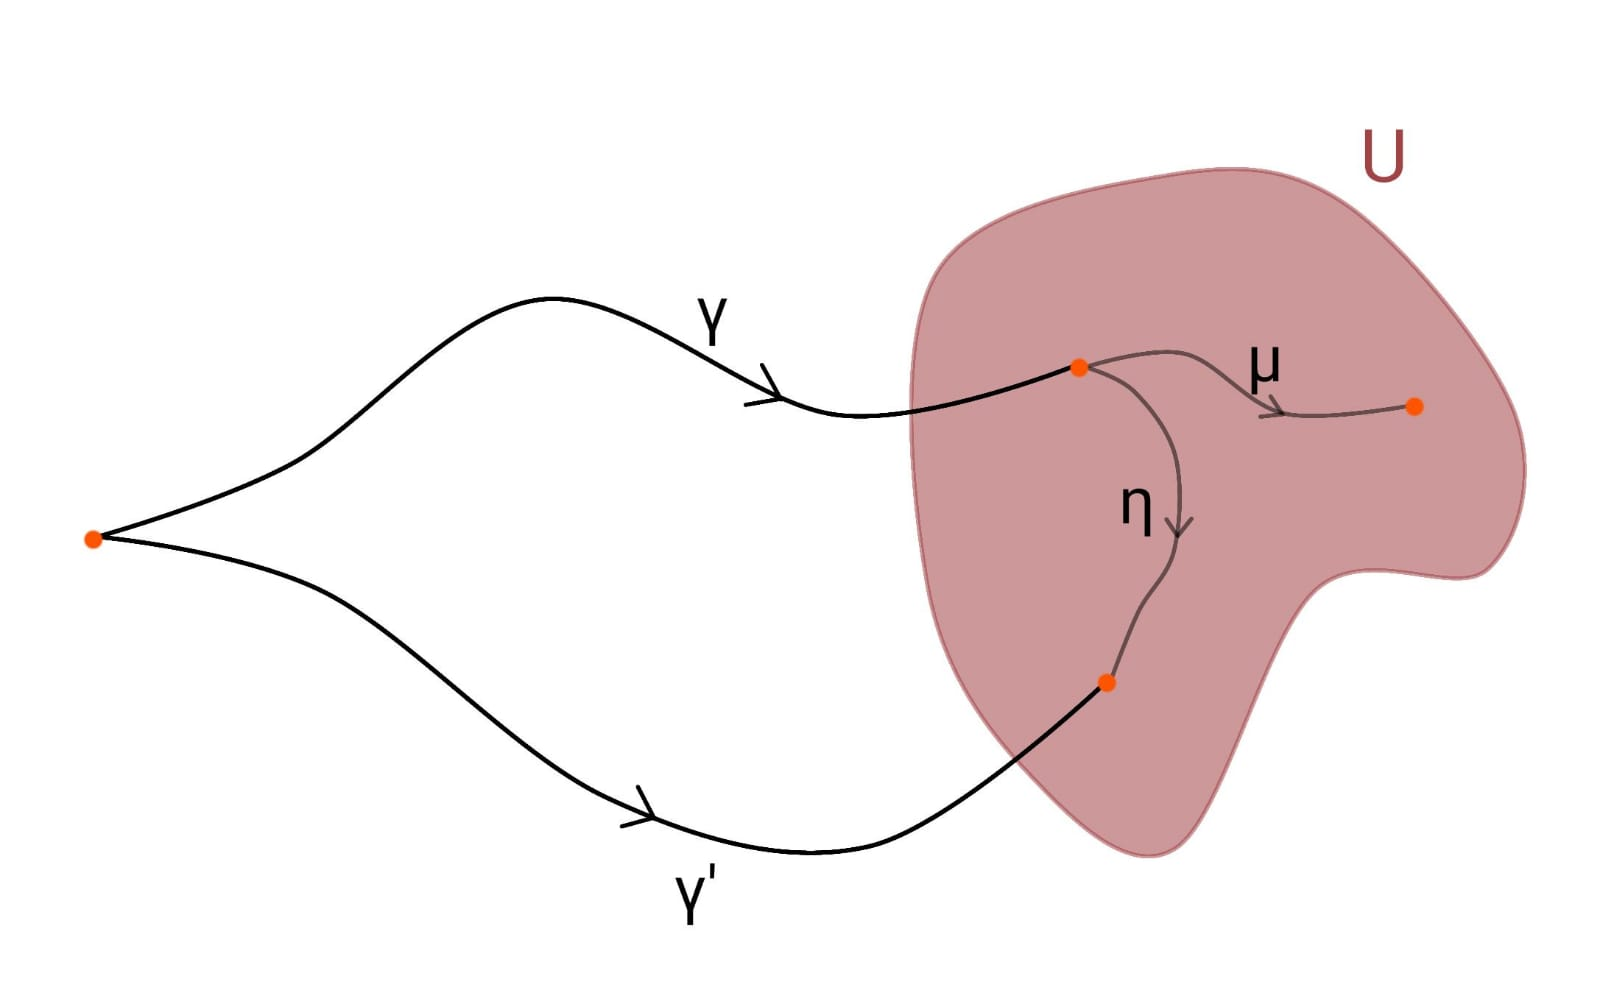
\includegraphics[width=0.8\linewidth]{conteudo/fig-cobertura-P(X,x_0).jpeg}
         \caption{Verificação de quando dois abertos $U_{[\gamma]}$ são iguais}
         \label{fig:cobertura-P(X,x_0)}
     \end{figure} 

     
     Verifiquemos que abertos desta forma constituem uma base para $P(X,x_0)$ e, além disso, que $q:U_{[\gamma]}\rightarrow U$ é um homeomorfismo, o que nos aproxima da verificação de que $q:P(X,x_0)\rightarrow X$ é um espaço de recobrimento.\newline

     De fato, temos as seguintes informações:

     \begin{enumerate}
        \item  $q:U_{[\gamma]}\rightarrow U$ é mapa injetor.\newline
        
        Escolhas diferentes de $\eta$ em $U$ que ligam $\gamma(1)$ a um mesmo ponto $x\in U$, isto é, dois caminhos $\eta_1$ e $\eta_2$ nessas condições tais que $q([\gamma*\eta_1])=q([\gamma*\eta_2])$, são tais que $\eta_1\sim \eta_2 (\text{rel }\partial I)$. Isso ocorre porque $i^*:\pi_1(U,x)\rightarrow \pi_1(X,x)$ é trivial, o que leva a conclusão de que dada a curva fechada $\eta_1* \overline{\eta_2}$ com ponto base $x$, temos a igualdade $[\eta_1* \overline{\eta_2}]=[c_x]\in \pi_1(X,x)$ e, portanto, $$\eta_1\sim\eta_1*(\overline{\eta_2}*\eta^2)\sim (\eta_1*\overline{\eta_2})*\eta^2\sim c_x*\eta_2\sim  \eta_2~(\text{rel }\partial I).$$  Dessa forma, $\gamma*\eta_1\sim \gamma*\eta_2 (\text{rel }\partial I)$ e, portanto, $[\gamma*\eta_1]=[\gamma*\eta_2]$. A situação é descrita na figura \ref{fig:restricao-de-q-é-injetor}.

        \begin{figure}[h!]
         \centering
         \includegraphics[width=0.8\linewidth]{conteudo/fig-restricao-de-q-é-injetor.jpeg}
         \caption{Restrição de $q$ a $U_{[\gamma]}$ é mapa injetor}
         \label{fig:restricao-de-q-é-injetor}
     \end{figure} 
     
         \item $q:U_{[\gamma]}\rightarrow U$ é mapa sobrejetor.\newline
         
         Como $U$ é conexo por caminhos, sempre é possível encontrar curva $\eta$ em $U$ que ligue $\gamma(1)$ a qualquer outro ponto de $U$.\newline
         
         \item $\tilde{\mathcal{B}}=\{U_{[\gamma]}|~U\in \mathcal{B}, \gamma:I\rightarrow X\text{ com }\gamma(0)=x_0\text{ e }\gamma(1)=x\in U\}$ é base para a topologia de $P(X,x_0)$.\newline
         
        Os abertos de $\tilde{\mathcal{B}}$ realmente cobrem $P(X,x_0)$ porque dado qualquer $[\gamma]\in P(X,x_0)$, se $\gamma(1)=x$, então existe $U\in \mathcal{B}$ vizinhança de $x$ de forma que $[\gamma]\in U_{[\gamma]}$.
        Além disso, dados $U_{[\gamma_1]} $ e $V_{\gamma_2}$ quaisquer em $\tilde{\mathcal{B}}$ e um elemento $[\gamma]\in U_{\gamma_1}\cap V_{\gamma_2}$, temos que $U_{[\gamma]}= U_{[\gamma_1]}$ e $V_{[\gamma]}=V_{[\gamma_2]}$, pois mostramos anteriormente que em geral $U_{[\gamma]}=U_{[\gamma']}$ se e somente se $[\gamma']\in U_{[\gamma]}$. Assim, $\gamma(1)\in U$, $\gamma(1)\in V$ e é possível tomar $W\in \mathcal{B}$ tal que $W\subset U\cap V$ é vizinhança de $\gamma(1)$, uma vez que $\mathcal{B}$ é base. Dessa forma, $W_{[\gamma]}\subset U_{[\gamma]}\cap V_{[\gamma]}=U_{[\gamma_1]}\cap V_{[\gamma_2]}$ pertence a $\tilde{\mathcal{B}}$ e contém $[\gamma]=[\gamma*c_{\gamma(1)}]$\newline
         

         \item $q:U_{[\gamma]}\rightarrow U$ é de fato homeomorfismo.\newline
         
            Seja $V\subset U$ aberto em $\mathcal{B}$. A pré-imagem desse aberto pela restrição de $q$ em $U_[\gamma]$ é $q^{-1}(V)\cap U_{[\gamma]}= V_{[\gamma']}$ para qualquer $[\gamma']\in U_{[\gamma]}$ tal que $\gamma'(1)\in V$, uma vez que $V_{[\gamma']} \subset U_{[\gamma']}=U_{[\gamma]}$ e já vimos que $q:V_{[\gamma']}\rightarrow V$ é uma bijeção. 
            
            De fato, se $V'\subset U$ é aberto qualquer, $V'=\underset{\lambda\in \Lambda, U_\lambda\in \mathcal{B}}{\bigcup} U_\lambda$ união enumerável de abertos e a pré imagem de $V'$ pela restrição de $q$ em $U_{[\gamma]}$ é $$q^{-1}(V')\cap U_{[\gamma]} =\underset{\lambda\in \Lambda, U_\lambda\in \mathcal{B}}{\bigcup} q^{-1}(U_\lambda)\cap U_{[\gamma]} = \underset{\lambda\in \Lambda, U_\lambda\in \mathcal{B}}{\bigcup} (U_\lambda)_{[\gamma_\lambda]}$$ para qualquer $[\gamma_\lambda]\in U_{[\gamma]}$ tal que $\gamma_\lambda(1)\in U_\lambda$. De fato, a pré-imagem é união enumerável de abertos e, portanto, aberta.
            
            
            Além disso, como $q(V_{[\gamma]})=V$ aberto e $\tilde{\mathcal{U}}$ é base, temos que dado qualquer aberto $V''\subset U_{[\gamma]}$ é $V''=\underset{\lambda \in \Lambda, U_\lambda \in \tilde{\mathcal{U}}}{\bigcup} U_\lambda$ união enumerável de abertos e então $q(V'')=\underset{\lambda \in \Lambda, U_\lambda \in \tilde{\mathcal{U}}}{\bigcup} q(U_\lambda)$, onde $q(U_\lambda)\in \mathcal{B}$ para todo $\lambda \in \Lambda$. Isto é, $q(V'')$ é união enumerável de abertos e, portanto, aberto.\newline

        \item $q:P(X,x_0)\rightarrow X$ é contínuo.\newline
        
            Para todo aberto $V\subset X$, temos que $V=\underset{\lambda\in \Lambda, V_\lambda \in \mathcal{B}}{\bigcup} V_\lambda$ para certos abertos $V_\lambda$ em $\mathcal{B}$.

            Temos que $$q^{-1}(V)=q^{-1}(\underset{\lambda\in \Lambda, V_\lambda \in \mathcal{B}}{\bigcup} V_\lambda)=\underset{\lambda\in \Lambda, V_\lambda \in \mathcal{B}}{\bigcup}q^{-1}(V_\lambda),$$ onde $q^{-1}(V_\lambda)=\underset{\gamma, (V_\lambda)_[\gamma] \in \tilde{\mathcal{B}}}{\bigcup} (V_\lambda)_{[\gamma]}$.

            Assim, todo $[\gamma]\in q^{-1}(V)$ é tal que $\gamma(1)\in V$ e, portanto, $\gamma(1)\in V_{\lambda_0}$ para algum $\lambda_0\in \Lambda$. Isto significa que $[\gamma]\in (V_{\lambda_0})_\gamma\subset q^{-1}(V)$ aberto. Portanto, $q^{-1}(V)$ é de fato aberto, como queríamos.\newline\newline
     \end{enumerate}


    Assim, temos que para todo $x\in X$ existe $U\in \mathcal{B}$ vizinhança de $x$ tal que  $p^{-1}(U)=\underset{[\gamma]}{\sqcup} U_{[\gamma]}$, onde cada $U_{[\gamma]}$ é homeomorfo a $U$. Essa união é disjunta pois se $U_{[\gamma_1]}\neq U_{[\gamma_2]}$ e $[\gamma]\in U_{[\gamma_1]}\cap U_{[\gamma_2]}$, então $U_{[\gamma]}=U_{[\gamma_1]}$ e $U_{[\gamma]}=U_{[\gamma_2]}$, o que implica $U_{[\gamma_1]}=U_{[\gamma_2]}$, uma contradição. Portanto, $U$ é aberto uniformemente recoberto de $X$ e isso conclui a nossa demonstração de que $P(X,x_0)$ é espaço de recobrimento.\newline

    Resta, por último, verificar que $P(X,x_0)$ é 1-conexo:

    \begin{enumerate}
        \item $P(X,x_0)$ é conexo por caminhos.\newline
        
            De fato, para todo $[\gamma]\in P(X,x_0)$, tome $\gamma_t:[0,1]\rightarrow X$ como a curva definida por 

            $$\begin{cases}
                \gamma(s), \text{ se }s\in [0,t]\\
                \gamma(t), \text{ se }s\in [t,1]
            \end{cases}$$

            Assim a curva $t\mapsto [\gamma_t]$ é um caminho em $P(X,x_0)$ que começa em $[c_{\gamma(0)}]=[c_{x_0}]$, curva constante em $\gamma(0)=x_0$, e termina em $[\gamma]$.

            Como isso vale para todo $[\gamma]$ em $P(X, x_0)$, então esse espaço é conexo por caminhos.\newline
        
        \item $\pi_1(P(X,x_0), [c_{x_0}])=0$\newline
        
            Para esta verificação mostraremos que $p_*: \pi_1(P(X,x_0), [c_{x_0}])\rightarrow \pi_1(X,x_0)$ é trivial.\newline

            Um elemento na imagem de $p_*$ é da forma $[\gamma]$ onde $\gamma$ é curva fechada com ponto base $x_0$ e seu levantamento também deve ser curva fechada, neste caso com ponto base $[c_{x_0}]$. Foi visto no item anterior que $t\mapsto [\gamma_t]$ levanta $\gamma$, começando em $[x_0]$ e terminando em $[\gamma_1]=[\gamma]$. Se esse levantamento é uma curva fechada, então $[\gamma]=[c_{x_0}]$ e o mapa de fato é trivial.

            Como $p_*$ é injetivo segundo o lema \ref{homomorfismo-induzido-por-recobrimento-prop}, então o fato de ser trivial implica $\pi_1(P(X,x_0), [c_{x_0}])=0$, como queríamos.\newline
        
    \end{enumerate}

    Assim, verificamos que $q: P(X,x_0)\rightarrow X$ é de fato um recobrimento 1-conexo e concluí-se por fim que, nas condições do enunciado, quando $X$ é semi-localmente simplesmente conexo, $X$ admite recobrimento 1-conexo.
    
\end{dem}

\begin{titlemize}{Lista de consequências}
	\item \hyperref[pertence-a-base-se-e-somente-se-possui-i-trivial]{Proposição - nova descrição da base $\mathcal{B}$};\\ %'consequencia1' é o label onde o conceito Consequência 1 aparece
    %\item \hyperref[espaço-1-conexo-def]{Espaço 1-conexo}
    \item \hyperref[recobrimento-universal]{Recobrimento universal}
\end{titlemize}

%---------------------------------------------------------------------------------------------------------------------!Draft!-----------------------------------------------------------------------------------------------------------------
\subsection{Descrição de $\tilde{\mathcal{B}}$ em termos de $X$} %afirmação aqui significa teorema/proposição/colorário/lema
\label{descrição-da-base-do-recobrimento-prop}
\begin{titlemize}{Lista de dependências}
	\item \hyperref[espaco-de-recobrimento-def]{Espaço de recobrimento};\\ %'dependencia1' é o label onde o conceito Dependência 1 aparece (--à arrumar um padrão para referencias e labels--) 
	\item \hyperref[espaço-1-conexo-def]{Espaço 1-conexo};\\
% quantas dependências forem necessárias.
\end{titlemize}


%Comentário sobre os objetos envolvidos na afirmação.



\begin{af}[Base para recobrimento 1-conexo]% ou af(afirmação)/prop(proposição)/corol(corolário)/lemma(lema)/outros ambientes devem ser definidos no preambulo de Alg.Top-Wiki.tex 
	Seja $p: E\rightarrow X$ um recobrimento com $X $ localmente conexo por caminhos e $E$ 1-conexo. A base $\tilde{\mathcal{B}}$ da topologia de $E$ definida em \ref{base-para-topologias-em-recobrimento-prop} pode ser descrita em termos de $X$ em dois casos:\newline

    \textbf{Caso 1:} Seja $U\in \mathcal{B}$ um aberto uniformemente recoberto com $x_0\in U$.\newline

    Em um espaço $\tilde{U}$ que seja placa de $U$ é possível levantar um caminho $\eta$ entre $x_0$ e $y_0$, em que $y_0\in U$ qualquer já que o espaço é conexo por caminhos, para um caminho $\tilde{\eta}$ entre $\tilde{x_0}$ e $\tilde{y_0}$ onde estes são pontos tais que $p(\tilde{x_0})=x_0$ e $p(\tilde{y_0})=y_0$.\newline

    Defina $U_{\tilde{x_0}}=\{\tilde{\eta}_{\tilde{x_0}}(1)|~\eta:I\rightarrow U\text{ e }\eta(0)=x_0\}$. A partir desta definição, é possível dizer que todas as placas de $U$ podem ser escritas como $U_{\tilde{x_0}}$ para algum $\tilde{x_0}$, que é o único valor existente na placa tal que $p(\tilde{x_0})=x_0$. Isto é,

    $$p^{-1}(U)=\underset{\tilde{x_0}\in p^{-1}(x_0)}{\sqcup} U_{\tilde{x_0}}$$
    


    \textbf{Caso 2:} Seja $U\subset X$ aberto conexo por caminhos e uniformemente recoberto, isto é, $U\in \mathcal{B}$. Tome $x\in U$ e seja $\tilde{x}\in E$ tal que $p(\tilde{x})=x$.\newline
    
    Fixe uma curva $\gamma: I\rightarrow X$ com $\gamma(0)=x_0$ e $\gamma(1)=x$, isto é, $[\gamma]\in q^{-1}(x)$. Note que $q$ é a função $q:P(X,x_0)\rightarrow X$ onde $P(X,x_0)=\{[\gamma]|~\gamma(0)=x_0\}$ definida por $q([\gamma])=\gamma(1)$.\newline
    
    Pode-se escrever $U$ como o espaço formado por $\gamma*\eta(1)$ para algum $\eta:I\rightarrow U$ tal que $\eta(0)=x$. Isto é, é possível descrever o aberto de $\tilde{\mathcal{B}}$ que é placa de $p$ sobre $U$ e vizinhança de $\tilde{x}$ como $$\tilde{U}_{\tilde{x}}=\{(\widetilde{\gamma*\eta})_{e_0}(1)|~\eta:I\rightarrow U,~\eta(0)=x\},$$ onde $e_0$ é tal que $\tilde{\gamma}_{e_0}(1)=\tilde{x}$.
    
    
    
	
\end{af}



\begin{titlemize}{Lista de consequências}
	\item \hyperref[pertence-a-base-se-e-somente-se-possui-i-trivial]{Proposição - nova descrição da base $\mathcal{B}$};\\ %'consequencia1' é o label onde o conceito Consequência 1 aparece
%	\item \hyperref[]{}
\end{titlemize}

%[Bianca]: Um arquivo tex pode ter mais de uma afirmação (ou definição, ou exemplo), mas nesse caso cada afirmação deve ter seu próprio label. Dar preferência para agrupar afirmações que dependam entre sí de maneira próxima (um teorema e seu corolário, por exemplo)
%---------------------------------------------------------------------------------------------------------------------!Draft!-----------------------------------------------------------------------------------------------------------------
\subsection{Base da topologia de $X$ possui $i^*$ trivial para todos os elementos quando há recobrimento 1-conexo} %afirmação aqui significa teorema/proposição/colorário/lema
\label{pertence-a-base-se-e-somente-se-possui-i-trivial}
\begin{titlemize}{Lista de dependências}
	\item \hyperref[base-para-topologias-em-recobrimento-prop]{Base para as topologias em um recobrimento};\\ %'dependencia1' é o label onde o conceito Dependência 1 aparece (--à arrumar um padrão para referencias e labels--) 
	\item \hyperref[recobrimento-1-conexo-prop]{Existe recobrimento 1-conexo se e somente se X slsc};\\
    \item \hyperref[descrição-da-base-do-recobrimento-prop]{Descrição de $\tilde{\mathcal{B}}$ em termos de $X$};\\
    \item \hyperref[1-conexo-prop]{Propriedades de 1-conexo};\\
    \item \hyperref[levantamento-de-homotopia-prop]{Levantamento de Homotopia}
% quantas dependências forem necessárias.
\end{titlemize}
%Comentário sobre os objetos envolvidos na afirmação.
\begin{prop}% ou af(afirmação)/prop(proposição)/corol(corolário)/lemma(lema)/outros ambientes devem ser definidos no preambulo de Alg.Top-Wiki.tex 
	Sejam $p:E\rightarrow X$ um recobrimento 1-conexo e $U\subset X$ um aberto conexo por caminhos. Então $U\in \mathcal{B}$, onde $\mathcal{B}$ é base para a topologia de $E$ conforme definida em \ref{base-para-topologias-em-recobrimento-prop}, se se somente se $i_*:\pi_1(U,x)\rightarrow \pi_1(X,x)$ é trivial.\\

\end{prop}
\begin{dem}
    Por um lado, se $U\in \mathcal{B}$ temos que, dada a inclusão $i:U\rightarrow X$, $i_*:\pi(U,x)\rightarrow \pi(X,x)$ é um mapa trivial segundo argumentação realizada no início da demonstração do Teorema \ref{recobrimento-1-conexo-prop}.\newline

    Por outro lado, se $i_*:\pi_1(U,x)\rightarrow \pi_1(X,x)$ é trivial, vamos verificar que $U$ é uniformemente recoberto. Em particular, verifiquemos que $p^{-1}(U)=\underset{[\gamma]\in q^{-1}(X)}{\bigsqcup} \tilde{U}_{[\gamma]}$ onde $$\tilde{U}_{[\gamma]}=\{(\widetilde{\gamma*\eta})_{\tilde{x}}(1)|~\eta:I\rightarrow U,~\eta(0)=x\}$$, da mesma forma que é descrito no "caso 2" da Afirmação \ref{descrição-da-base-do-recobrimento-prop}. Isto é, $\tilde{U}_{[\gamma]}\in \tilde{B}$.

    Para tal, verifiquemos:

    \begin{enumerate}
        \item $\tilde{U}_{[\gamma]}\subset p^{-1}(U)$ para todo $[\gamma]$ pois
        $$p(\tilde{U}_{[\gamma]})=\{p((\widetilde{\gamma*\eta})_{\tilde{x}}(1))|~\eta:I\rightarrow U,~\eta(0)=x\}=$$$$=\{(\gamma*\eta)(1)|~\eta:I\rightarrow U,~\eta(0)=x\}=\{\eta(1)\in U|~\eta:I\rightarrow U,~\eta(0)=x\}\subset U$$\newline

        \item $p^{-1}(U)\subset \underset{[\gamma]\in q^{-1}(x)}{\bigcup} \tilde{U}_{[\gamma]}$

        Seja $\tilde{y}\in p^{-1}(U)$, seja $\eta:I\rightarrow U$ com $\eta(0)=x$ e $\eta(1)=y=p(\tilde{y})$ e seja $\tilde{x}=\tilde{\overline{\eta}}_{\tilde{y}}(1)$, de forma que $p(\tilde{x})=x$.

        Seja $ \xi:I\rightarrow E$ com $\xi(0)=e_0$, $\xi(1)=\tilde{x}$ e seja $\gamma=p\circ \xi$. Então $ \tilde{y}\in \tilde{U}_{[\gamma]}$ pois $(\widetilde{\gamma * \eta})_{e_0}(1)=\tilde{\eta}_{\tilde{x}}(1)=\tilde{y}$.\newline

        \item Se $[\gamma_0]\neq [\gamma_1]\in q^{-1}(x)$, então $ \tilde{U}_{[\gamma_0]}\cap \tilde{U}_{[\gamma_1]}=\emptyset$

        Suponha que $\tilde{y}\in \tilde{U}_{[\gamma_0]}\cap\tilde{U}_{[\gamma_1]}$. Sejam $\eta_0, \eta_1: I\rightarrow U$ curvas tais que $(\widetilde{\gamma_0*\eta_0})_{e_0}(1)=(\widetilde{\gamma_1*\eta_1})_{e_0}(1)=\tilde{y}$, como representado na figura \ref{fig:classes-distintas-de-curvas} a seguir.

\begin{figure}[h!]
         \centering
         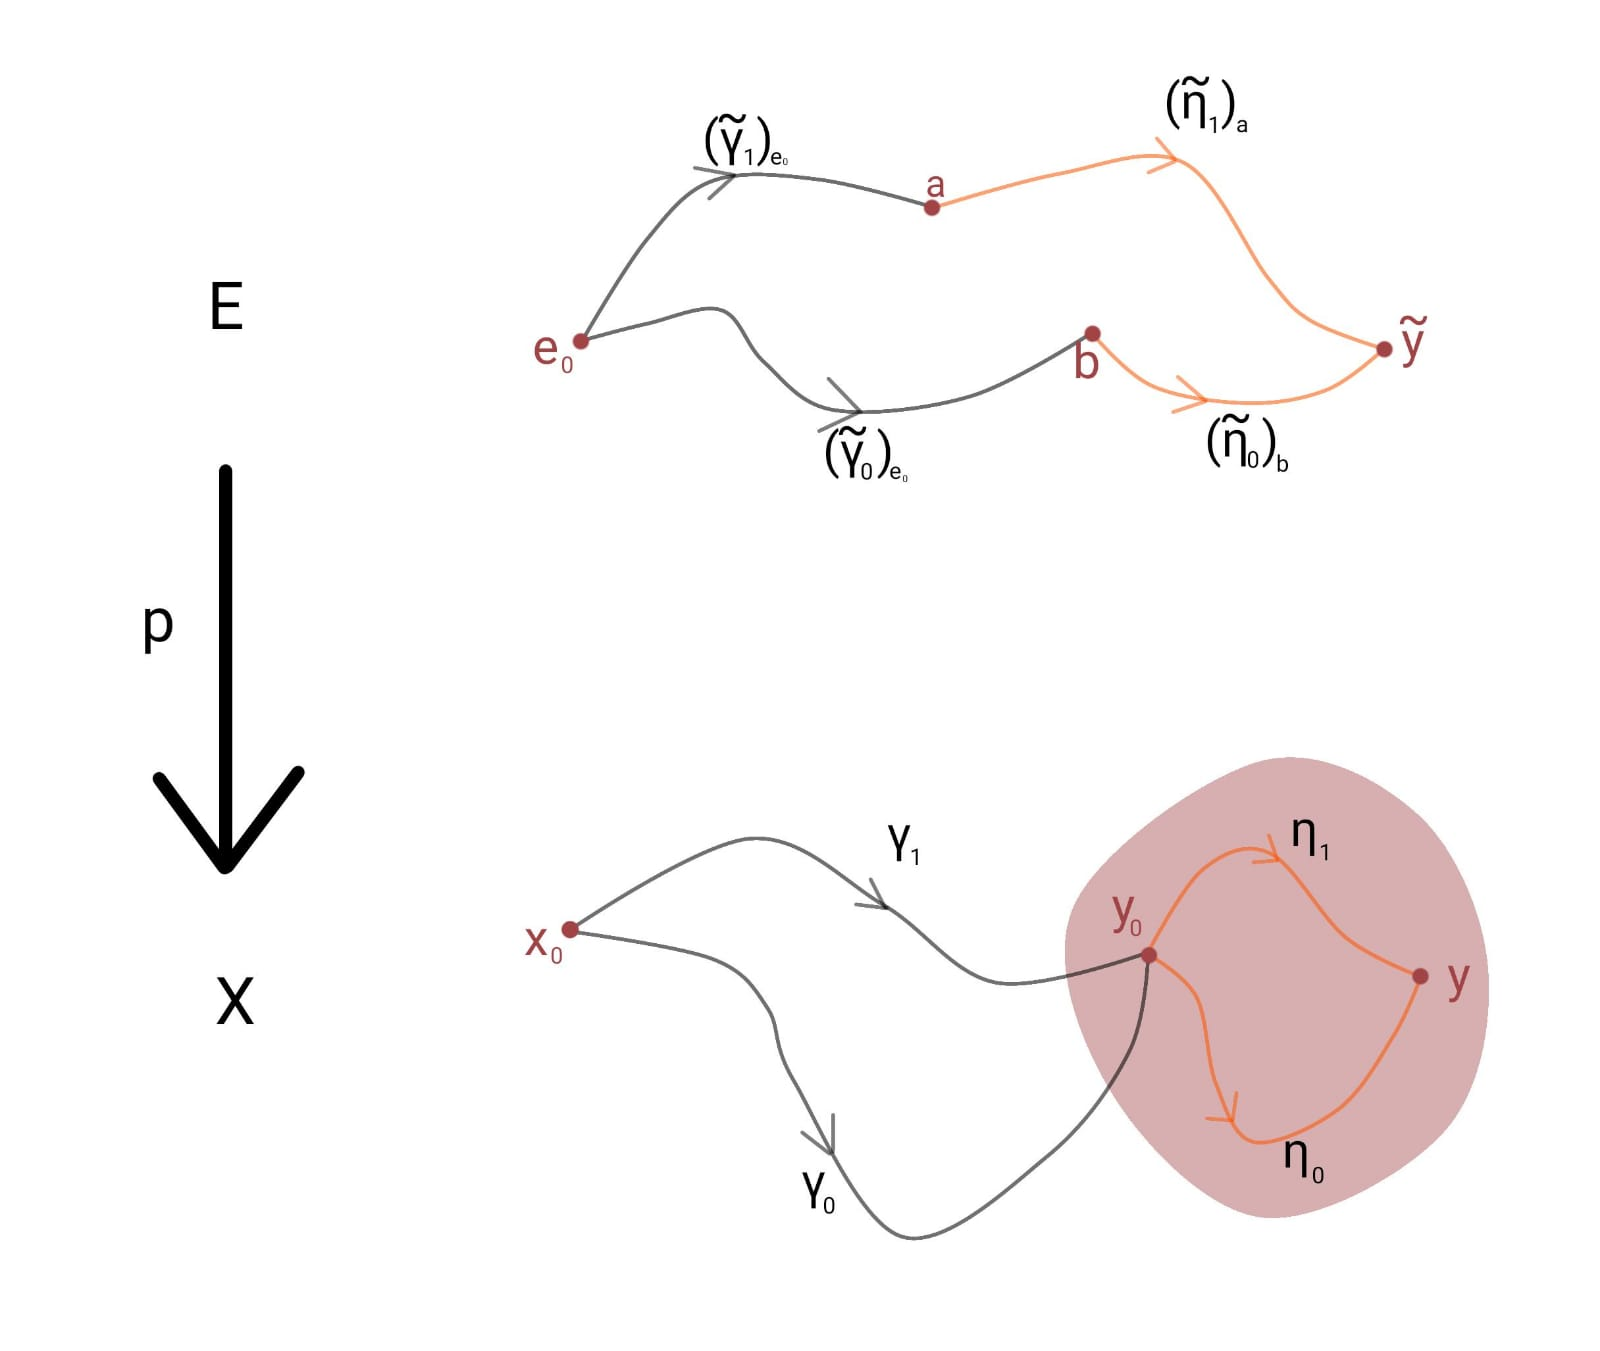
\includegraphics[width=0.8\linewidth]{conteudo/fig-classes-distintas-de-curvas.jpeg}
         \caption{Classes distintas de curvas, mas $\tilde{y}$ na intersecção dos abertos}
         \label{fig:classes-distintas-de-curvas}
     \end{figure} 

        
        Assim, temos que $p\circ(\widetilde{\gamma_0*\eta_0})_{e_0}(1)=y=p\circ(\widetilde{\gamma_1*\eta_1})_{e_0}(1)$ e portanto $\eta_0(1)=y=\eta_1(1)$.

        Na mesma figura, é possível notar que $\eta_0*\overline{\eta}_1$ é um laço em $U$ com ponto base $y$. Como nos foi dado que $i^*:\pi(U,x)\rightarrow \pi_1(X,x)$ é trivial e $U$ conexo por caminhos, temos que

        $$(\eta_0*\overline{\eta}_1)\sim c_y~(\text{rel}~\partial I) \Rightarrow (\widetilde{\eta_0 * \overline{\eta_1}})_{\tilde{y}}\sim  c_{\tilde{y}}~(\text{rel}~\partial I)\Rightarrow (\tilde{\gamma}_0)_{e_0}(1)=(\tilde{\gamma}_1)_{e_0}(1),$$ diferentemente do que a imagem indica.

        Como $E$ é 1-conexo, utilizando a Proposição \ref{1-conexo-prop} concluí-se que $[\gamma_0]=[\gamma_1]$, um absurdo por contradizer a hipótese inicial.\newline
        

    
        \item A restrição $p|_{\tilde{U}_{[\gamma]}}:\tilde{U}_{[\gamma]}\rightarrow U $ é bijeção

        Para verificar a sobrejetividade basta notar que para todo $y\in U$ é possível tomar a curva $\eta:I\rightarrow U$ tal que $\eta(0)=x$ e $\eta(1)=y$. Temos que se $\tilde{y}=(\widetilde{\gamma*\eta})_{e_0}(1)\in \tilde{U}_{[\gamma]}$, então $p(\tilde{y})=y$, como queríamos.

        Para a verificação da injetividade, basta supor que $p((\widetilde{\gamma*\eta_0})_{e_0}(1))=p((\widetilde{\gamma*\eta_1})_{e_0}(1))$ onde $\eta_0, \eta_1:I\rightarrow U$ são tais que $\eta_0(0)=x=\eta_1(0)$ e $\eta_0(1)=\eta_1(1)$. Portanto, $\eta_0*\overline{\eta}_1$ é laço e assim $\eta_0\sim \eta_1~(\text{rel }\partial I)$.
        Isso significa que, se $\tilde{x}=\tilde{\gamma}_{e_0}(1)$, então $(\tilde{\eta}_0)_{\tilde{x}}(1)= (\tilde{\eta}_1)_{\tilde{x}}(1)$ segundo Corolário presente em \ref{levantamento-de-homotopia-prop}. Assim, $(\widetilde{\gamma*\eta_0})_{e_0}(1)=(\gamma*\eta_1)_{e_0}(1)$.\newline

        \item A restrição $p|_{\tilde{U}_{[\gamma]}}$ é aplicação aberta pois $\tilde{U}_{[\gamma]}\in \tilde{\mathcal{B}}$ é uma placa do recobrimento.\newline
    \end{enumerate}

    Assim, verificamos que $U$ é uniformemente recoberto, isto é, $U \in \mathcal{B}$ como queríamos.\newline
\end{dem}

O resultado acima implica que a base $\mathcal{B}$ pode ser descrita como $\mathcal{B}=\{U\subset X|~U\text{ é conexo por caminhos e }i_*:\pi_1(U,x)\rightarrow \pi_1(X,x)\text{ é trivial}\}$

%\begin{titlemize}{Lista de consequências}
%	\item \hyperref[consequencia1]{Consequência 1};\\ %'consequencia1' é o label onde o conceito Consequência 1 aparece
%	\item \hyperref[]{}
%\end{titlemize}

%[Bianca]: Um arquivo tex pode ter mais de uma afirmação (ou definição, ou exemplo), mas nesse caso cada afirmação deve ter seu próprio label. Dar preferência para agrupar afirmações que dependam entre sí de maneira próxima (um teorema e seu corolário, por exemplo)

%%% Local Variables:
%%% mode: LaTeX
%%% TeX-master: "../Alg.Top-Wiki"
%%% End:
